\documentclass[a4paper,11pt]{article}
\usepackage[margin=25mm]{geometry}
\usepackage{fontspec}
\usepackage{polyglossia}
\setdefaultlanguage{russian}
\setotherlanguage{english}
\setmainfont{Liberation Serif}
\setsansfont{Liberation Sans}
\setmonofont{DejaVu Sans Mono}[Scale=0.82]
\usepackage{amsmath,amssymb,amsthm,graphicx,booktabs}
\usepackage[hidelinks,unicode]{hyperref}
\setlength{\emergencystretch}{3em}
\newtheorem{theorem}{Теорема}[section]
\newtheorem{lemma}[theorem]{Лемма}
\newtheorem{proposition}[theorem]{Утверждение}
\newtheorem{corollary}[theorem]{Следствие}
\hypersetup{pdftitle={Гарантированная остановка метода Франка-Вульфа при ненулевом градиенте в минимуме},pdfauthor={Ярослав П. Ляхов и Степан А. Суворов}}
\title{Гарантированная остановка метода Франка-Вульфа\\при ненулевом градиенте в минимуме}
\author{Ярослав П. Ляхов \and Степан А. Суворов}
\date{12 ноября 2026}
\begin{document}
\maketitle
\begin{abstract}
В минимуме на множестве градиент может оставаться сколь угодно большим.
Рассматриваются остановка и выбор шага для выпуклых функций на компактных
выпуклых множествах при гладкости, зависящей от градиента. Сертификат
по полному зазору и квадратичный подбор шага дают конечную остановку
без знания значения минимума и без стремления нормы градиента к нулю.
Подсчитаны запросы градиента и линейного оракула, отклонённые пробы
функции и адаптивные уточнения направленных данных. Для областей в
форме прямого произведения добавление нормального линейного слагаемого
не меняет выполнение метода, начатого на соответствующей грани.
На глобально $(1,1)$-гладком семействе $e^x+Ay$ фиксированное правило шага
через норму градиента требует не менее порядка $A$ шагов, а подбор шага
не зависит от $A$. Детерминированный эксперимент воспроизводит это
различие при одинаковом сертификате остановки.
\end{abstract}
\section{Введение}
\label{sec:intro}
Мы рассматриваем минимизацию выпуклой функции на компактном выпуклом
множестве $Q$. Функция дважды непрерывно дифференцируема в окрестности
$Q$ и удовлетворяет условию гладкости
\[
 \|\nabla^2 f(x)\|\le L_0+L_1\|\nabla f(x)\|,\qquad x\in Q.
\]
Параметры $L_0,L_1$ и диаметр $Q$ входят в оценку числа запросов;
самому методу с подбором шага их значения не нужны.
Неизвестное минимальное значение не входит ни в условие гладкости,
ни в алгоритм. Точка $x^*$ обозначает минимум только в анализе.

Полный зазор Франка-Вульфа
$G(x)=\max_{s\in Q}\langle\nabla f(x),x-s\rangle$
в силу выпуклости удовлетворяет
$f(x)-f(x^*)\le G(x)$ \cite{jaggi}.
Поэтому $f(x)-G(x)$ даёт вычисляемую нижнюю границу минимума.
Оценка верна и для граничного решения с ненулевым градиентом.
Остановку определяет зазор, а не требование малой нормы градиента.

При этом зависимость кривизны от градиента влияет на выбор шага.
Мы показываем этот эффект на семействе выпуклых функций
\[
 f_A(x,y)=\exp(x)+Ay,\qquad
 Q=[-1,1]\times[0,1],\qquad A>0.
\]
Все функции имеют одни и те же параметры $L_0=L_1=1$.
При старте из $(0.7,0)$ полный линейный оракул всегда возвращает
$(-1,0)$. Зазор и значения функции вдоль посещаемой грани не зависят
от $A$, хотя норма градиента растёт вместе с $A$.
Мы доказываем, что шаг из алгоритма~1 Выгузова и Стонякина
\cite{vyguzov} с фиксированными параметрами гладкости требует
$\Omega(A)$ обновлений даже для пересечения прямой $x=0$.
При точных ответах оракула и одинаковой начальной оценке кривизны
квадратичный бэктрекинг даёт одни и те же пробные точки, принятые
шаги и число запросов до остановки при всех $A$.
Сравнение относится к их алгоритму~1 с фиксированными параметрами.
Оно не распространяется на адаптивный алгоритм~2.

Далее строится правило остановки с адаптивной абсолютной точностью
направленного оракула. Границы его ошибки подтверждают и полный
зазор, и величину спуска вдоль выбранного направления.
Запрошенная точность переносится между итерациями и уточняется при
необходимости. Алгоритм сохраняет лучшую подтверждённую нижнюю
границу минимума. Доказана остановка с заданной ошибкой по функции
и получены оценки всех вызовов оракула и вычислений функции.
Подсчёт включает неудачные проверки точности, отклонённые пробные
шаги и заключительную проверку остановки. Точные градиенты и точная
линейная минимизация по всему $Q$ входят в эту схему как частный случай.

\paragraph{Связь с известными результатами.}
Сертификаты через зазор и неточные линейные оракулы уже входят в
анализ выпуклого метода Франка-Вульфа \cite{jaggi}.
Выгузов и Стонякин \cite{vyguzov} изучают фиксированные и адаптивные
шаги при указанном условии гладкости.
Квадратичный бэктрекинг также известен \cite{pedregosa}.
Мы используем этот способ шага и доказываем приведённые выше гарантии
остановки с полным подсчётом запросов. Явное семейство количественно
показывает, как компонента градиента влияет на шаг через норму,
хотя выбранное направление и значения функции вдоль него не меняются.

Условие кривизны через невязку функции из анализа разогрева шага
\cite{warmup} является другой моделью и здесь не предполагается.
Метод Local LMO \cite{locallmo} минимизирует линейную функцию
по $Q\cap B(x,t)$, а наше правило сохраняет полный линейный оракул
по $Q$. Таким образом, используется исходная выпуклая постановка,
без регулярности относительно неизвестного центра и без знания
$f(x^*)$.

\section{Постановка и доступные вычисления}
\label{sec:model}
Пусть $Q\subset\mathbb R^d$ является непустым компактным выпуклым
множеством, $\operatorname{diam}Q\le D$, $D>0$. Функция $f$ выпукла
на $Q$ и дважды непрерывно дифференцируема в его окрестности. Предположим
\begin{equation}\label{eq:gradient_smoothness}
 \|\nabla^2f(x)\|\le L_0+L_1\|\nabla f(x)\|,\qquad x\in Q,
 \quad L_0,L_1\ge0.
\end{equation}
Для векторов используется евклидова норма, для матриц спектральная.
Минимизатор $x^*\in Q$ существует. Он нужен для записи гарантии
точности, но не подаётся на вход метода. Выражения $f(x)-f(x^*)$ и
$\|\nabla f(x)\|$ записываем полностью, без отдельных обозначений.

Доступны вычисление функции, вычисление градиента и линейная
минимизация по всему $Q$. Последняя возвращает
\[
 s\in\arg\min_{v\in Q}\langle\nabla f(x),v\rangle.
\]
Полный зазор Франка-Вульфа вычисляется по формуле
\begin{equation}\label{eq:gap}
 G(x)=\max_{v\in Q}\langle\nabla f(x),x-v\rangle
     =\langle\nabla f(x),x-s\rangle.
\end{equation}
Поскольку $x\in Q$, имеем $G(x)\ge0$. Из выпуклости следует
$f(x)-f(x^*)\le G(x)$, поэтому $f(x)-G(x)$ даёт нижнюю границу
неизвестного минимума \cite{jaggi}. Сам минимум при проверке остановки
вычислять не требуется.

В минимуме на множестве выполняется условие
\[
 \langle\nabla f(x^*),v-x^*\rangle\ge0\quad(v\in Q).
\]
Оно равносильно $G(x^*)=0$ и не требует $\nabla f(x^*)=0$.
Например, $f(x)=Ax+x^2/2$ на $[0,1]$, $A>0$, имеет минимум в нуле,
производную $A$ в этой точке и гессиан, равный единице.
Большой градиент и большая кривизна являются разными свойствами.

\begin{lemma}[Конечная граница кривизны по начальному градиенту]
\label{lem:global_curvature}
Из условия гладкости следует
\begin{equation}\label{eq:global_curvature}
 \|\nabla^2f(z)\|\le K_Q\quad(z\in Q),\qquad
 K_Q=(L_0+L_1\|\nabla f(x_0)\|)e^{L_1D}.
\end{equation}
В результатах ниже вместо $K_Q$ можно использовать любую более точную
равномерную верхнюю границу. Эта константа нужна для оценки числа
вычислений; алгоритму знать её не требуется.
\end{lemma}
\begin{proof}
Для единичного направления $e$ вдоль отрезка из $x_0$ внутри $Q$
основная теорема анализа даёт
\[
 \|\nabla f(x_0+te)\|\le\|\nabla f(x_0)\|
 +\int_0^t\{L_0+L_1\|\nabla f(x_0+se)\|\}\,ds.
\]
При $L_1>0$ неравенство Гронуолла ограничивает
$L_0+L_1\|\nabla f(x_0+te)\|$ величиной
$(L_0+L_1\|\nabla f(x_0)\|)e^{L_1t}$. Остаётся учесть $t\le D$.
При $L_1=0$ исходное условие сразу даёт границу $L_0$.
\end{proof}

Условие гладкости не содержит неизвестного минимума. Алгоритм ниже
также не требует константы регулярности относительно неизвестного
минимизатора или его удалённости от границы. Полный зазор ограничивает
глобальную ошибку благодаря выпуклости функции.

\section{Остановка с гарантией точности и подбором шага}
\label{sec:stopping}
Предположим, что выполнены условия выпуклой модели из
раздела~\ref{sec:model}. Из выпуклости следует
\begin{equation}\label{eq:gap_certificate}
 f(x)-f(x^*)\le
 \langle\nabla f(x),x-x^*\rangle\le G(x).
\end{equation}
Полный зазор даёт вычисляемую границу ошибки и при
$\nabla f(x^*)\ne0$. Оценивать этот неизвестный градиент не нужно.
В доказательстве используем положительную границу кривизны $K_Q$
из \eqref{eq:global_curvature}. Если она равна нулю, её можно
увеличить до любого положительного числа. Сам алгоритм не требует
заданных значений $K_Q$, $L_0$ или $L_1$.

\paragraph{Алгоритм с точными оракулами.}
Зададим $\varepsilon>0$ и начальное значение кривизны
$L_{\rm init}>0$. В текущей точке $x$ вычисляем градиент,
линейный минимум $s\in Q$ и зазор $G(x)$. Сохраняем
\[
 \ell\leftarrow\max\{\ell,f(x)-G(x)\},
\]
причём первый запрос задаёт $\ell=f(x_0)-G(x_0)$.
Если $f(x)-\ell\le\varepsilon$, останавливаемся.
Иначе берём $d=s-x$, начинаем с половины ранее принятой кривизны
(начальное сохранённое значение равно $L_{\rm init}$) и удваиваем
$L$, пока не выполнится
\begin{equation}\label{eq:stopping_bt}
 \alpha=\min\left\{1,\frac{G(x)}{L\|d\|^2}\right\},\qquad
 f(x+\alpha d)\le f(x)-\alpha G(x)+\frac{L\alpha^2\|d\|^2}{2}.
\end{equation}
Принимаем $x+\alpha d$, сохраняем значение функции и принятое $L$.
Это обычный подбор шага метода Франка-Вульфа \cite{pedregosa}.
Значения функции, градиенты и линейные минимумы на всём $Q$ точны.

\begin{theorem}[Конечная остановка и число всех запросов]
\label{thm:finite_stopping}
Каждый подбор шага завершается. Алгоритм останавливается с
$f(x_N)-f(x^*)\le f(x_N)-\ell_N\le\varepsilon$.
Если $G(x_0)>\varepsilon$, положим
\[
 J=\left\lceil\log_2\frac{G(x_0)}{\varepsilon}\right\rceil,
 \quad b_j=G(x_0)/2^j\ (0\le j<J),
\]
\[
 H_{\rm init}=\left\lceil
 \log_2\max\left\{1,\frac{L_{\rm init}}{2K_Q}\right\}\right\rceil.
\]
Число $N$ принятых шагов удовлетворяет
\begin{align}
 N&\le H_{\rm init}+\left\lceil\sum_{j=0}^{J-1}
       \max\left\{4,\frac{16K_QD^2}{b_j}\right\}\right\rceil
       \label{eq:stopping_steps}\\
  &\le H_{\rm init}+\left\lceil4J+
       \frac{32K_QD^2}{\varepsilon}\right\rceil.
       \label{eq:stopping_simple}
\end{align}
Вычислений градиента и запросов линейной минимизации ровно по $N+1$,
включая последний запрос. Начальное значение функции и все принятые
и отклонённые пробы при подборе шага дают не более
\begin{equation}\label{eq:stopping_values}
 N_f\le 1+2N+
 \left\lceil\log_2\max\left\{1,\frac{2K_Q}{L_{\rm init}}\right\}\right\rceil
\end{equation}
вычислений функции.
Если $G(x_0)\le\varepsilon$, шагов нет, а каждый из трёх оракулов
вызывается ровно один раз; величины для фаз не нужны.
\end{theorem}

\begin{proof}
Каждая сохранённая $\ell$ ограничивает $f(x^*)$ снизу, поэтому
\[
 0\le f(x)-f(x^*)\le f(x)-\ell\le G(x).
\]
В нетерминальной точке $G(x)>0$ и $d\ne0$.
Любое $L\ge K_Q$ проходит проверку \eqref{eq:stopping_bt}.
Для принятых значений выполнено
\begin{equation}\label{eq:stopping_progress}
 \begin{split}
 L_k&\le\max\{L_{k-1}/2,2K_Q\},\qquad L_{-1}=L_{\rm init},\\
 f(x_k)-f(x_{k+1})&\ge
 \min\left\{\frac{G(x_k)}2,\frac{G(x_k)^2}{2L_kD^2}\right\}.
 \end{split}
\end{equation}
Значение функции убывает, $\ell$ возрастает, а $f(x_k)-\ell_k$
убывает. Если $L_k>2K_Q$, была принята первая проба: иначе
предыдущая отклонённая проба $L_k/2>K_Q$ тоже прошла бы проверку.
Такой шаг делит сохранённую кривизну пополам. После достижения
$L_k\le2K_Q$ эта граница сохраняется. Шагов выше этого порога
не больше $H_{\rm init}$.

Каждый оставшийся нетерминальный шаг отнесём к фазе
$b_j/2<f(x_k)-\ell_k\le b_j$. Фазы посещаются по порядку.
В фазе $j$ зазор больше $b_j/2$, и \eqref{eq:stopping_progress}
даёт уменьшение функции не меньше
\[
 \min\left\{b_j/4,\ b_j^2/(16K_QD^2)\right\}.
\]
Суммарное уменьшение на всех шагах, начинающихся в этой фазе,
не больше истинной ошибки при входе в неё, то есть не больше $b_j$.
Сюда входит и последний шаг, выводящий из фазы: в его конечной
точке функция не меньше $f(x^*)$. Деление и суммирование доказывают
\eqref{eq:stopping_steps}. Из $\sum_{j<J}b_j^{-1}<2/\varepsilon$
следует \eqref{eq:stopping_simple}. Та же конечная граница верна
для каждого незавершённого начала процесса, поэтому бесконечный
процесс без остановки невозможен.

Если на шаге $k$ отклонены $q_k$ проб, то
$L_k=2^{q_k-1}L_{k-1}$. При $N\ge1$ получаем
\[
 \sum_{k<N}(q_k+1)=2N+\log_2\frac{L_{N-1}}{L_{\rm init}},
 \quad L_{N-1}\le\max\{L_{\rm init}/2^N,2K_Q\}.
\]
Добавление начального значения функции даёт
\eqref{eq:stopping_values}. В каждой посещённой точке нужен один
градиент и одно решение задачи линейной минимизации.
\end{proof}

\subsection{Перенос направленной точности между итерациями}
Направленный запрос с требуемой точностью $\eta>0$ возвращает
$h\ge0$ и $d=s-x$, $s\in Q$, с гарантированными границами
\begin{equation}\label{eq:directional_query}
 G(x)\le h+\eta,\qquad
 -\langle\nabla f(x),d\rangle\ge h-\eta.
\end{equation}
Это явное требование к оракулу. Проверка при подборе шага сама
по себе его не доказывает. Значения функции остаются точными.
Основной алгоритм с точными оракулами этого дополнения не требует.

Начнём с $\eta_0>0$ и зададим $0<\theta<1$.
После каждого запроса обновляем
$\ell\leftarrow\max\{\ell,f(x)-(h+\eta)\}$ и сначала проверяем
$f(x)-\ell\le\varepsilon$. Если остановки нет и $\eta>\theta h$,
делим $\eta$ пополам и повторяем запрос в той же точке, сохраняя
её значение функции. Когда $\eta\le\theta h$, используем
\eqref{eq:stopping_bt}, заменив $G(x)$ на $h-\eta$.
В следующую точку переносим достигнутую $\eta$.

\begin{corollary}[Учёт всех уточнений точности]
\label{cor:directional_stopping}
Правило останавливается с $f(x_N)-f(x^*)\le\varepsilon$.
Положим $\kappa=(1-\theta)/(1+\theta)$. Общее число $R$ делений
точности пополам удовлетворяет
\begin{equation}\label{eq:accuracy_refinements}
 R\le\left\lceil\log_2\max\left\{1,
 \frac{(1+\theta)\eta_0}{\theta\varepsilon}\right\}\right\rceil.
\end{equation}
Если первая верхняя граница зазора $h_0+\eta_0>\varepsilon$,
определим $J$ и $b_j$ как выше, заменив $G(x_0)$ на $h_0+\eta_0$.
Тогда
\begin{equation}\label{eq:directional_steps}
 N\le H_{\rm init}+\left\lceil
 \frac{4J}{\kappa}+\frac{32K_QD^2}{\kappa^2\varepsilon}
 \right\rceil.
\end{equation}
Направленных запросов ровно $N+1+R$. Граница
\eqref{eq:stopping_values} для вычислений функции сохраняется.
Если каждый направленный запрос использует один линейный минимум
на всём $Q$, таких вызовов тоже $N+1+R$.
Если первая граница зазора не больше $\varepsilon$, правило
останавливается сразу.
\end{corollary}
\begin{proof}
При неудачной проверке точности без остановки
\[
 \varepsilon<f(x)-\ell\le h+\eta
 <(1+\theta)\eta/\theta.
\]
Так как $\eta$ делится пополам и не увеличивается, получаем
\eqref{eq:accuracy_refinements}. При успешной проверке без остановки
\[
 h-\eta\ge\kappa(h+\eta)\ge\kappa(f(x)-\ell)>0.
\]
Предыдущее доказательство уменьшения и подсчёта шагов применимо
с порогом направленного спуска $\kappa b_j/2$, что даёт
\eqref{eq:directional_steps}. В каждой посещённой точке есть один
завершающий запрос, включая последнюю точку, а каждое деление
точности добавляет один неудачный запрос. При уточнении в одной
точке значение функции повторно не вычисляется.
\end{proof}

Доказательство остановки использует полный зазор и допускает
ненулевой предельный градиент. В разделе~\ref{sec:normal} и точная
граница кривизны, и всё выполнение метода не зависят от сколь угодно
большой нормальной компоненты градиента. Число направленных запросов
указывает, как часто нужна заданная точность; стоимость получения
каждого ответа определяется реализацией оракула.

\section{Большой нормальный градиент и неизменная траектория}
\label{sec:normal}
Правая часть условия гладкости может расти из-за линейного слагаемого,
которое не меняет кривизну. Следующее утверждение описывает семейство,
для которого такой рост не влияет на метод с подбором шага.

\begin{proposition}[Неизменность метода при нормальном линейном слагаемом]
\label{prop:normal_invariance}
Пусть $Q_0$ компактно и выпукло, а $\varphi$ выпукла и принадлежит
$C^2$ в окрестности $Q_0$. Для $A\ge0$ рассмотрим
\[
 Q=Q_0\times[0,1],\qquad f_A(z,y)=\varphi(z)+Ay.
\]
Запустим точный метод раздела~\ref{sec:stopping} из $(z_0,0)$ с
одинаковыми точностью и начальной кривизной. При неоднозначности
выбираем один и тот же линейный минимум на $Q_0$, а по координате $y$
выбираем ноль. Тогда для всех $A\ge0$ совпадают точки, зазоры,
принятые шаги, пробы подбора шага и числа обращений к оракулам.
Если $\varphi$ удовлетворяет~\eqref{eq:gradient_smoothness}, то
каждая $f_A$ удовлетворяет ему с теми же константами. В минимуме
$(z^*,0)$ имеем
\[
 \|\nabla f_A(z^*,0)\|
   =\sqrt{\|\nabla\varphi(z^*)\|^2+A^2}\ge A.
\]
\end{proposition}
\begin{proof}
В точке $(z,0)$ градиент равен $(\nabla\varphi(z),A)$. Поэтому полный
линейный оракул возвращает $(s,0)$, где $s$ минимизирует
$\langle\nabla\varphi(z),s\rangle$ на $Q_0$.
Последняя координата направления равна нулю. Его норма, направленная
производная, зазор и все значения функции вдоль него не зависят от $A$.
Значит, совпадают сохраняемая нижняя граница и все проверки шага.
Индукция доказывает совпадение всего выполнения алгоритма.
Гессиан состоит из блока $\nabla^2\varphi$ и нулевого блока, а
$\|\nabla f_A\|\ge\|\nabla\varphi\|$, что доказывает утверждение о
гладкости.
\end{proof}

Верхняя граница $\|\nabla^2\varphi\|$ на $Q_0$ даёт значение $K_Q$,
не зависящее от $A$, для теоремы~\ref{thm:finite_stopping}.
Таким образом, и выполнение метода, и верная оценка числа шагов
могут не зависеть от этой нормальной компоненты.
Обратная матрица Гессе нигде не используется.

\subsection{Сравнение с шагом по фиксированным параметрам гладкости}
Правило из Algorithm~1 работы~\cite{vyguzov} имеет вид
\begin{equation}\label{eq:vyguzov_step}
 \alpha_k=\min\left\{1,
 \frac{G(x_k)}{e(L_0+L_1\|\nabla f(x_k)\|)\|s_k-x_k\|^2}
 \right\}.
\end{equation}
Здесь $e$ является основанием натурального логарифма. Сравниваем с
подбором шага именно это правило. Адаптивный Algorithm~2 из той же
работы является другим методом.

\begin{theorem}[Линейное различие по нормальному коэффициенту]
\label{thm:normal_separation}
Пусть
\[
 f_A(x,y)=e^x+Ay,\qquad Q=[-1,1]\times[0,1],\qquad A>0.
\]
Начальная точка равна $(a,0)$, где $0<a<1$, и
$0<\varepsilon<1-e^{-1}$. В правиле~\eqref{eq:vyguzov_step} положим
$L_0=L_1=1$ и используем тот же критерий остановки с сохраняемой
нижней границей, что и в разделе~\ref{sec:stopping}. До остановки
этому правилу требуется не менее
\begin{equation}\label{eq:normal_lower}
 \left\lceil a e^{1-a}A\right\rceil
\end{equation}
шагов. Выполнение метода с подбором шага, включая конечный момент
остановки, не зависит от $A$.
\end{theorem}
\begin{proof}
Функции выпуклы на всей плоскости, причём
\[
 \nabla f_A(x,y)=(e^x,A),\qquad
 \nabla^2f_A(x,y)=\operatorname{diag}(e^x,0).
\]
Поэтому условие~\eqref{eq:gradient_smoothness} выполнено всюду с
одними и теми же $L_0=L_1=1$. Минимум на $Q$ находится в $(-1,0)$.
Полный линейный оракул всегда возвращает $(-1,0)$. Точки остаются
на $y=0$, а первая координата убывает. В текущей координате $x$
зазор равен $e^x(x+1)$. Правило~\eqref{eq:vyguzov_step} уменьшает
координату не более чем на
\[
 \frac{e^x}{e(1+\sqrt{e^{2x}+A^2})}
 \le\frac{e^a}{eA}.
\]
Оценка остаётся верной и при ограничении шага единицей. Пока
координата не стала отрицательной, истинная ошибка не меньше
$1-e^{-1}>\varepsilon$, поэтому верный сертификат не допускает
остановку. Требуется пройти расстояние не меньше $a$, откуда
следует~\eqref{eq:normal_lower}.
Независимость подбора шага от $A$ доказана в
утверждении~\ref{prop:normal_invariance}. Его конечная остановка
следует из теоремы~\ref{thm:finite_stopping}, например при $K_Q=e$
и $D=\sqrt5$. Обе константы не зависят от $A$.
\end{proof}

Результат относится к конкретному выпуклому семейству и указанному
правилу шага. Причина видна в~\eqref{eq:vyguzov_step}: нормальная
компонента входит в знаменатель, хотя не меняет ни функцию вдоль
сделанных шагов, ни гессиан. Подбор шага проверяет фактическое
изменение функции вдоль направления.

\section{Воспроизводимый эксперимент с граничным минимумом}
\label{sec:experiments}
Для семейства из теоремы~\ref{thm:normal_separation} взяты $a=0.7$,
$\varepsilon=10^{-6}$, $L_{\rm init}=1$ и
$A\in\{0,1,10,100,1000\}$. Сравниваются
правило~\eqref{eq:vyguzov_step} при $L_0=L_1=1$ и точный метод
с подбором шага. Оба метода сохраняют одну и ту же нижнюю границу
для проверки остановки. Полный линейный оракул на прямоугольнике
использует фиксированный выбор при равенстве значений.
Во всех десяти запусках нет случайности и подбора параметров.

\begin{table}[htbp]
\centering
\caption{Принятые шаги и вычисления функции. Каждый запуск с подбором
шага использует три градиента и три полные линейные минимизации.}
\label{tab:boundary}
\begin{tabular}{rrrrr}
\toprule
$A$ & Фикс. шаг & Подбор шага & Фикс. $N_f$ & Подбор $N_f$\\
\midrule
0    & 11   & 2 & 12   & 5\\
1    & 14   & 2 & 15   & 5\\
10   & 66   & 2 & 67   & 5\\
100  & 610  & 2 & 611  & 5\\
1000 & 6045 & 2 & 6046 & 5\\
\bottomrule
\end{tabular}
\end{table}

Все запуски останавливаются в $(-1,0)$ с нулевым зазором.
Траектории подбора шага полностью совпадают для всех пяти значений
$A$: первая принятая кривизна равна двум, вторая единице; всего
отклонены две пробы. При $A=1000$ норма градиента в решении примерно
равна $1000.000068$, а ошибка по функции и сертификат равны нулю.

\begin{figure}[htbp]
\centering
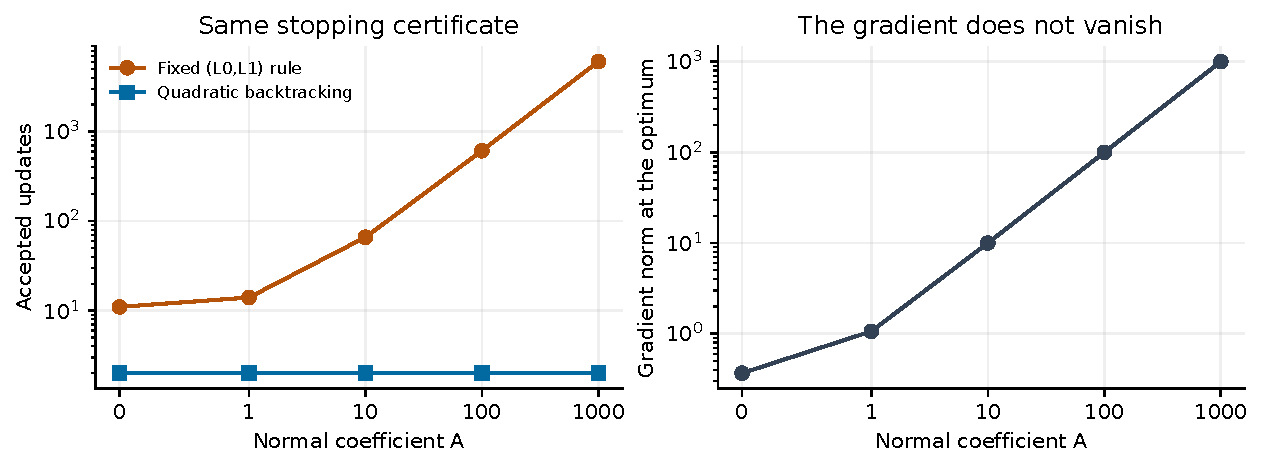
\includegraphics[width=\linewidth]{../figures/boundary_normal_benchmark.pdf}
\caption{Фиксированный шаг через норму градиента уменьшается с ростом
нормального коэффициента. Подбор шага выполняет те же два шага,
хотя градиент в минимуме неограниченно растёт.}
\label{fig:boundary}
\end{figure}

Скрипт \texttt{Code/benchmark\_boundary.py} сохраняет каждую посещённую
точку, зазор, накопленный сертификат, принятую кривизну и число
вызовов. Он проверяет допустимость точек, уменьшение функции,
аналитическую границу~\eqref{eq:normal_lower} и совпадение траекторий
подбора шага. Известное решение используется только для контрольной
проверки после остановки. Алгоритм не получает ни минимизатор,
ни значение минимума. В эксперименте используется арифметика Python
с плавающей точкой; утверждения разделов~\ref{sec:stopping}
и~\ref{sec:normal} доказаны независимо от численных проверок.

\paragraph{Смысл результата.}
Полный зазор даёт корректную остановку в граничном минимуме.
Подбор шага не зависит от нормального коэффициента в семействе из
утверждения~\ref{prop:normal_invariance}. В таблице~\ref{tab:boundary}
использован фиксированный Algorithm~1 работы~\cite{vyguzov};
доказательство и таблица относятся к одному и тому же сравнению.

\paragraph{Вычислительные инструменты.}
Инструменты ИИ использовались при выводах, проверках, подготовке кода
и текста. За проверку математических утверждений, источников и
вычислений отвечают авторы.

\begin{thebibliography}{99}
\bibitem{jaggi}M.~Jaggi.
Revisiting Frank-Wolfe: Projection-Free Sparse Convex Optimization.
\emph{Proceedings of the 30th International Conference on Machine Learning},
PMLR 28(1):427-435, 2013.
\url{https://proceedings.mlr.press/v28/jaggi13.html}.

\bibitem{vyguzov}A.~A.~Vyguzov and F.~S.~Stonyakin.
Frank-Wolfe Algorithms for $(L_0,L_1)$-smooth functions.
\href{https://arxiv.org/abs/2510.16468v5}{arXiv:2510.16468v5}, 2026.

\bibitem{pedregosa}F.~Pedregosa, G.~Negiar, A.~Askari, and M.~Jaggi.
Linearly Convergent Frank-Wolfe with Backtracking Line-Search.
\emph{Proceedings of the Twenty Third International Conference on
Artificial Intelligence and Statistics}, PMLR 108:1-10, 2020.
\url{https://proceedings.mlr.press/v108/pedregosa20a.html}.

\bibitem{warmup}F.~Alimisis, R.~Islamov, and A.~Lucchi.
Why Do We Need Warm-up? A Theoretical Perspective.
\href{https://arxiv.org/abs/2510.03164v2}{arXiv:2510.03164v2}, 2026.

\bibitem{locallmo}P.~Richt\'{a}rik, K.~Gruntkowska, and H.~Li.
Local LMO: Constrained Gradient Optimization via a Local Linear
Minimization Oracle.
\href{https://arxiv.org/abs/2605.08850v1}{arXiv:2605.08850v1}, 2026.
\end{thebibliography}

\end{document}
